\documentclass[a4paper, 12pt]{article} % тип документа

%%%Библиотеки
	%\usepackage[warn]{mathtext}	
	\usepackage[T2A]{fontenc}   %Кодировка
	\usepackage[utf8]{inputenc} %Кодировка исходного текста
	\usepackage[english, russian]{babel} %Локализация и переносы
	\usepackage{caption}
	\usepackage{gensymb}
	%\usepackage{listings}
	\usepackage{amsmath, amsfonts, amssymb, amsthm, mathtools}
	%\usepackage[warn]{mathtext}
	%\usepackage[mathscr]{eucal}
	%\usepackage{wasysym}
	%\usepackage{graphicx} %Вставка картинок правильная
	%\usepackage{pgfplots}
	\usepackage{indentfirst}
	%\usepackage{float}    %Плавающие картинки
	%\usepackage{wrapfig}  %Обтекание фигур (таблиц, картинок и прочего)
	\usepackage{fancyhdr} %Загрузим пакет
	%\usepackage{lscape}
	%\usepackage{xcolor}
	%\usepackage[normalem]{ulem}
	
	\usepackage{titlesec}
	\titlelabel{\thetitle.\quad}

	\usepackage{hyperref}

%%%Конец библиотек

%%%Настройка ссылок
	\hypersetup
	{
		colorlinks = true,
		linkcolor  = blue,
		filecolor  = magenta,
		urlcolor   = blue
	}
%%%Конец настройки ссылок


%%%Настройка колонтитулы
	\pagestyle{fancy}
	\fancyhead{}
	\fancyhead[L]{1.3.3}
	\fancyhead[R]{Глаз Роман, группа Б01-007}
	\fancyfoot[C]{\thepage}
%%%конец настройки колонтитулы



\begin{document}
						%%%%Начало документа%%%%


%%%Начало титульника
\begin{titlepage}

	\newpage
	\begin{center}
		\normalsize Московский физико-технический институт \\(госудраственный университет)
	\end{center}

	\vspace{6em}

	\begin{center}
		\Large Лабораторная работа по общему курсу физики\\Термодинамика и молекулярная физика
	\end{center}

	\vspace{1em}

	\begin{center}
		\Large \textbf{1.3.3. Измерение вязкости воздуха по течению в тонких трубках }
	\end{center}

	\vspace{2em}

	\begin{center}
		\large Глаз Роман Сергеевич\\
		Группа Б01-007
	\end{center}

	\vspace{\fill}

	\begin{center}
	Долгопрудный \\2021
	\end{center}
	
\end{titlepage}
%%%Конец Титульника



%%%Настройка оглавления и нумерации страниц
	\thispagestyle{empty}
	\newpage
	\tableofcontents
	\newpage
	\setcounter{page}{1}
%%%Настройка оглавления и нумерации страниц


					%%%%%%Начало работы с текстом%%%%%%

\textbf{Цель работы:} экспериментально исследовать свойства течения газов по тонким трубкам при различных числах Рейнольдса; выявить область применимости закона Пуазейля и с его помощью определить коэффициент вязкости воздуха.\\

\textbf{Используемое оборудование:} система подачи воздуха (компрессор, поводящие трубки); газовый счетчик барабанного типа; спиртовой микроманометр с регулируемым наклоном; набор трубок различного диаметра с выходами для подсоединения микроманометра; секундомер.

\section{Теоретические сведения}

\subsection{Теория}

Рассмотрим движение вязкой жидкости или газа по трубке круглого сечения. При малых скоростях потока движение оказывается ламинарным (слоистым), скорости частиц меняются по радиусу и направлены вдоль оси трубки. С увеличением скорости потока движение становится турбулентным, и слои перемешиваются. При турбулентном движении скорость в каждой точке быстро меняет величину и направление, сохраняется только средняя величина скорости.

Характер движения газа (или жидкости) в трубке определяется безразмерным числом Рейнольдса:

\begin{equation}
	Re = \dfrac{\upsilon r \rho}{\eta} \text{  } \text{  } \text{  }
\end{equation}

где $\upsilon$ - скорость потока, $r$ - радиус трубки, $\rho$ - плотность движущейся среды, $\eta$ - вязкость. В гладких трубах круглого сечения переход от ламинарного движения к турбулентному происходит при $Re \approx 1000$.

При ламинарном течении объем газа $V$, протекающий за время $t$ по трубе длиной $l$, определяется формулой Пуазейля:

\begin{equation}
	Q_V = \dfrac{\pi r^4}{8 l \eta}(P_1 - P_2) \text{  } \text{  } \text{  }
\end{equation}

В этой формуле $P_1 - P_2$ - разность давлений в двух выбранных сечениях $1$ и $2$, расстояние между которыми равно $l$. Велечину $Q$ обычно называют расходом. Формула (2) позволяет определять вязкость газа по его расходу.

Отметим условия, при которых справедлива формула (2). Прежде всего необходимо, чтобы с достаточным запасом выполнялось неравенство $Re < 1000$. Необходимо также, чтобы при течении не происходило существенного изменения удельного объема газа (при выводе формулы удельный объем считался постоянным). Для жидкости это предположение выполняется практически всегда, а для газа -- лишь в тех случаях, когда перепад давлений вдоль трубки мал по сравнению с самим давлением. В нашем случае давление газа равно атмосферному ($10^3$ см вод. ст.), а перепад давлений составляет не более 10 см вод. ст., то есть менее $1\%$ от атмосферного. Формула (2) выводится для участков трубки, на которых закон распределения скоростей газа по сечению не меняется при движении вдоль потока.

\begin{center}
		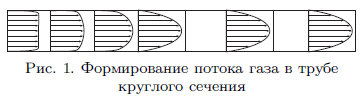
\includegraphics[width = 0.6\textwidth]{133_1}
\end{center}

При втекании газа в трубку из большого резервуара скорости слоев вначале постоянны по всему сечению (рис. 1). По мере продвижения газа по трубке картина распределения скоростей меняется, так как сила трения о стенку тормозит прилежащие к ней слои. Характерное для ламинарного течения параболическое распределение скоростей устанавливается на некотором расстоянии $a$ от входа в трубку, которое зависит от радиуса трубки $r$ и числа Рейнольдса по формуле

\begin{equation}
	l \approx  0,2 r \cdot Re \text{ } \text{ } \text{ }
\end{equation}

Градиент давления на участке формирования потока оказывается большим, чем на участке с установившимся ламинарным течением, что позволяет разделить эти участки экспериментально. Формула (3) дает возможность оценить длину участка формирования.


\subsection{Экспериментальная установка}

\begin{center}
    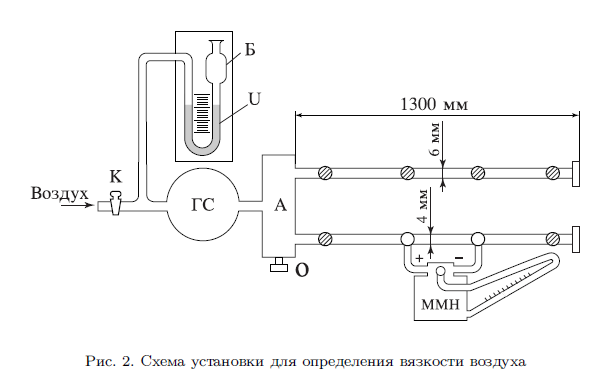
\includegraphics[width = \textwidth]{133_2.png}
\end{center}

Измерения производятся на экспериментальной установке, схема которой изображена на рис. 2. Поток воздуха под давлением, несколько превышающим атмосферное (на $5-7$ см вод. ст.), через газовый счетчик ГС поступает в резервуар А, к которому припаяны тонкие металлические трубки. Примерные размеры трубок указаны на рисунке (точные размеры обозначены на установке). Обе трубки на концах снабжены заглушками, не пропускающими воздух. Во время измерений заглушка открывается только на рабочей трубке; конец другой трубки должен быть плотно закрыт. Перед входом в газосчётчик поставлена U-образная трубка, наполовину заполненная водой. Она выполняет две задачи. Первая -- измерение давления газа на входе в газосчётчик. Вторая -- предохранение газосчётчика от выхода из строя. Дело в том, что газосчётчик устойчиво работает, если давление газа на его входе не превышает $600$ мм водяного столба. Высота U-образной трубки примерно $600$ мм, поэтому, когда давление на входе в счётчик превышает $600$ мм водяного столба,вода из U-образной трубки выплёскивается в защитный баллон Б и, создавая шум, привлекает к себе внимание экспериментатора.
 
\section{Ход работы}

\subsection{Предварительные оценки}

Найдём расход газа, при котором число Рейнольдса становится критическим. Для предварительной оценки примем значение взякости равным $\eta = 2 \cdot 10^{-5}$ $\text{Па} \cdot \text{с}$.

\begin{equation}
	Q_{cr} = u_{cr} \frac{\pi d^2}{4} = \frac{Re \cdot \eta}{\rho d} \frac{\pi d^2}{4} = Re \cdot \eta_{cr} \frac{\pi d}{4 \rho } = 0,065 \; \text{л/с}
\end{equation}

Здесь была взята величина плотности воздуха при нормальных условиях $\rho = 1,2 \; \text{кг}/\text{м}^3$.

Теперь из найденного насхода и формулы Пуазёйля найдём критическое давление:

\begin{equation}
	P_{cr} = \frac{8 \eta l}{\pi r^4} Q_{cr} \simeq 40 \; \text{Па}
\end{equation}

В качестве значения длины было взято значение $l = 0,5$ м.

Теперь оценим хаарктерную  длину установления ламинарного течения: по формуле (3) оцениваем расстояние, на котором происходит формирование потока при ламинарном течении. Расчет проведим для $Re = 1000$: $l \approx 0,39$ м.

Проверим полученные оценки на корректность: меняя расход воздуха краном К и наблюдая за столбиком спирта в микроманометре, визуально определим границу перехода от ламинарного течения к турбулентному. Проведя измрения для диаметра $d = 5$ мм имеем следующее значение, при котором наблюдаются пуульсации давления (хоть и совсем небольшие): $P_{cr} = 50 \; \text{мм пр. ст.} =  78$ Па -- значение близко к расчитанному теоретически.

\subsection{Предварительные расчёты}

Для начала определим, какими должны быть значения $\Delta V$ и $\Delta t$, чтобы рассчитанное значение расхода газа имело погрешность не более $1\%$.
 
\begin{equation}
	Q = \frac{\delta V}{\delta t} \Rightarrow \frac{\Delta Q}{Q} =  \left( \frac{\Delta V}{\delta V} + \frac{\Delta t}{\delta t} \right) \leqslant 0,01
\end{equation}

\begin{center}
	\begin{tabular}{|c|c|c|c|c|c|c|c|c|}
		\hline
		$dV$, л & 3     & 3     & 3     & 3     & 3     & 3     & 3     & 3     \\ \hline
		$dt$, с & 51,64 & 51,82 & 51,51 & 51,61 & 51,63 & 51,71 & 51,66 & 51,92 \\ \hline
	\end{tabular}
\end{center}

Согласно описанию установки, класс точности установки равен $1.0$, значит погрешность определения объёма равна $\Delta V = 0,05$ л.

Измерим случайную погрешность определения времени человеком с помощью секундомера. Для этого составим таблицу измеренных данных, измеряя время прохождения 3 л воздуха:

Имеем корень из дисперсии $\Delta t = 0,120$ с.

Из полученных значений следует, что объёму $6-7$ л и времени $30$ с соответсвует значение относительной погрешности менее $0,01$. Значит измеряемые данные должны иметь характерные величины.

\subsection{Исследование зависимости P(Q)}

Подготавливаем установку к работе: устанавливаем приборы по уровням, проверяем наличие воды в газовом счетчике по водомерному устройству, установливаем на ноль мениск микроманометра. Полный объём измерения проводим на одной из трубок (на трубке $d = 4$ мм).

Подсоединяем микроманометр к двум соседним выводам выбранной трубки на участке со сформировавшимся потоком. Отвинчиваем пробку на конце этой трубки; все остальные выводы на трубках плотно завинчены пробками, снабженными резиновыми прокладками.

Медленно открывая кран К (рис. 2) и впуская воздух в установку, внимательно следим за показаниями микроманометра.

Измеряем вязкость воздуха. По полученным данным строим график $\Delta P = f(Q)$. Из формулы (2) видно, что при ламинарном потоке зависимость $\Delta P$ от $Q$ должна быть линейной. При возникновении турбулентности линейность графика нарушается: разность давлений растет быстрее, чем расход газа.

\begin{table}[!h]
\begin{tabular}{|c|c|c|c|c|c|c|}
\hline
$Q$, л/с      & 0,0196   & 0,0365   & 0,0581                & 0,0694                & 0,0781               & 0,0932                \\ \hline
$P$, мм сп ст & 17       & 32       & 49                    & 60                    & 68                    & 84                    \\ \hline
$P$, Па       & 26,683  & 50,227  & 76,910               & 94,176   & 106,732              & 131,846              \\ \hline
$Q$, л/с      & 0,0998   & 0,104    & 0,112                 & 0,114                 & 0,119                 & 0,1265                \\ \hline
$P$, мм сп ст & 97       & 111      & 128                   & 144                   & 167                   & 199                   \\ \hline
$P$, Па       & 152,251 & 174,226 & 200,909              & 226,022 & 262,123              & 312,350              \\ \hline
$Q$, л/с      & 0,1341    & 0,1420    & \multicolumn{1}{l|}{} & \multicolumn{1}{l|}{} & \multicolumn{1}{l|}{} & \multicolumn{1}{l|}{} \\ \hline
$P$, мм сп ст & 229      & 257      & \multicolumn{1}{l|}{} & \multicolumn{1}{l|}{} & \multicolumn{1}{l|}{} & \multicolumn{1}{l|}{} \\ \hline
$P$, Па       & 359,438 & 403,387 & \multicolumn{1}{l|}{} & \multicolumn{1}{l|}{} & \multicolumn{1}{l|}{} & \multicolumn{1}{l|}{} \\ \hline
\end{tabular}
\end{table}

\begin{figure}[!h]
    \centering
    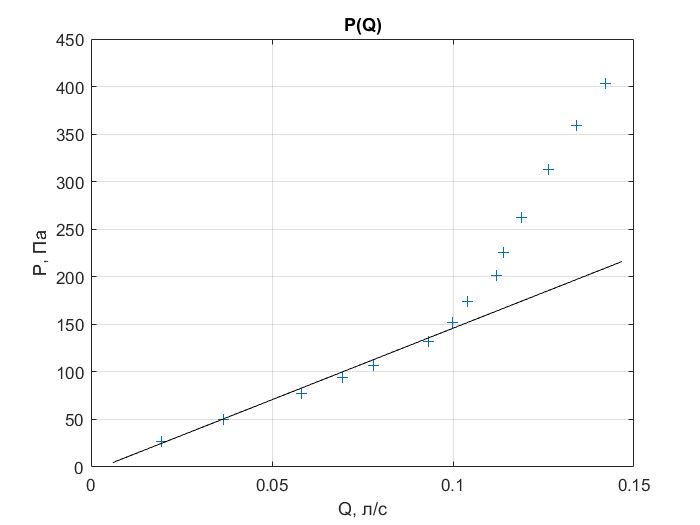
\includegraphics[width = 12 cm]{4mm}
    \caption{P(Q) для трубки 4 мм диаметром}
    \label{fig:vac}
\end{figure}

C помощью метода наименьших квадратов найдём угловой коэффициент для начальной части графика, где наблюдается лиинейная зависимость (первые 7 точек):

\begin{equation}
	\frac{8\eta l}{\pi r^4} = 1406 \; \text{Па} \cdot \text{c/л}, \; \Delta \left( \frac{8\eta l}{\pi r^4} \right) = 19 \; \text{Па} \cdot \text{c/л}
\end{equation}

\begin{equation}
	\eta = 1,759 \cdot 10^{-5} \; \text{Па} \cdot \text{c}, \; \frac{\Delta \eta}{\eta} = \frac{\Delta \frac{8\eta l}{\pi r^4}}{\frac{8\eta l}{\pi r^4}} +  \frac{\Delta l}{l} + 4 \frac{\Delta r}{r} = 0,028
\end{equation}

Табличное значение вязкости воздуха при температуре во время проведения эксперимента $t = 21 \; C^{\circ}$ равно $\eta = 1,78 \cdot 10^{-5} \; \text{Па} \cdot \text{c}$. То есть мы получили значение, совпадающее в пределах погрешности с теоретическим.

Границу перехода от ламинарного участка к турбулентному равна $P_{cr} = 200$ Па, что по порядку величины совпадает с ранее оценённым давлением (но там диаметр не 4, а 5 мм).

Вычислим значение числа Рейнольдса $Re$ для переходной области между ламинарным и турбулентным течениями:

\begin{equation}
	Re = \frac{4 \rho Q_{cr}}{\pi d \eta} \simeq 2400
\end{equation}

Получилась хорошая оценка числа Рейнольдса, совпадающая по порядку величины с ожидаемым значением-оценкой.

Проделаем те же самые действия для трубы двух других значений диаметра.

Для самой тонкой трубки $d = 3$ мм имеем следующие данные:

\begin{table}[]
\begin{tabular}{|c|c|c|c|c|c|c|}
\hline
$Q$, л/с      & 0,0101  & 0,0250   & 0,0342  & 0,0460    & 0,0559   & 0,0648   \\ \hline
$P$, мм сп ст & 15       & 34      & 51       & 71       & 97       & 118      \\ \hline
$P$, Па       & 23,544   & 53,366 & 80,049  & 111,441 & 152,251 & 185,212 \\ \hline
$Q$, л/с      & 0,0753   & 0,0813  & 0,0939  & 0,1001      & 0,1066   &          \\ \hline
$P$, мм сп ст & 146      & 170     & 208      & 241      & 268      &          \\ \hline
$P$, Па       & 229,161 & 266,832 & 326,477 & 378,274 & 420,653 &          \\ \hline
\end{tabular}
\end{table}

\begin{figure}[!h]
    \centering
    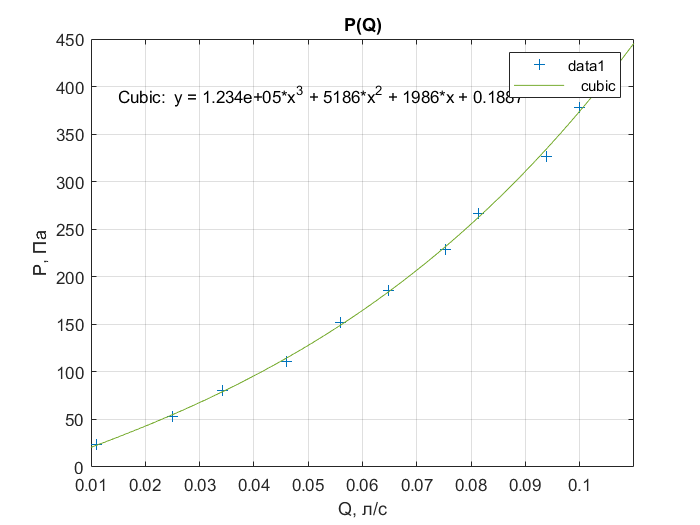
\includegraphics[width = 12 cm]{3mm}
    \caption{P(Q) для трубки 3 мм диаметром}
    \label{fig:vac}
\end{figure}

В данном случае участок перехода с ламинарного течения на турбулентное уже не так заметен. Построим прямую через начальные точки: 

\begin{figure}[!h]
    \centering
    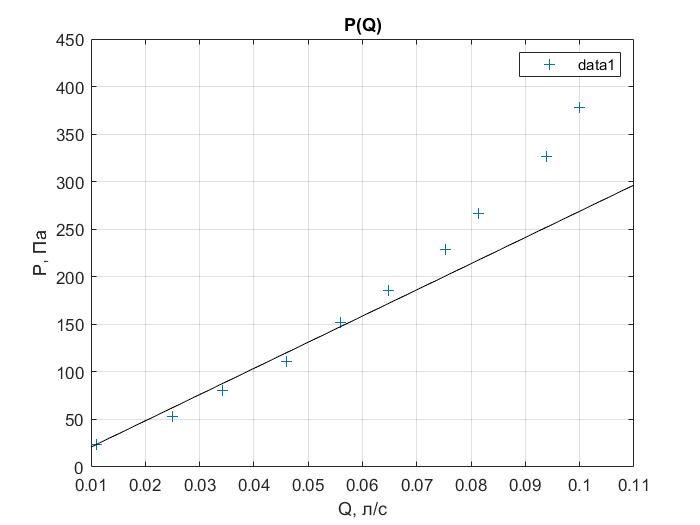
\includegraphics[width = 12 cm]{3mm2}
    \caption{P(Q) для трубки 3 мм диаметром}
    \label{fig:vac}
\end{figure}

Видно, что следует учитывать первые 6 точек для ламинарного течения. Найдём из МНК значение вязкости:

\begin{equation}
	\frac{8\eta l}{\pi r^4} = 3387 \; \text{Па} \cdot \text{c/л}, \; \Delta \left( \frac{8\eta l}{\pi r^4} \right) = 58 \; \text{Па} \cdot \text{c/л}
\end{equation}

\begin{equation}
	\eta = 1,744 \cdot 10^{-5} \; \text{Па} \cdot \text{c}, \; \frac{\Delta \eta}{\eta} = \frac{\Delta \frac{8\eta l}{\pi r^4}}{\frac{8\eta l}{\pi r^4}} +  \frac{\Delta l}{l} + 4 \frac{\Delta r}{r} = 0,054
\end{equation}

Значение получено верное в пределах погрешности, коэффициент корреляции равен $0,989$, что хорошо согласуется с количеством выбранных точек.

Границу перехода от ламинарного участка к турбулентному равна $P_{cr} = 200$ Па, что по порядку величины совпадает с ранее оценённым давлением.

Вычислим значение числа Рейнольдса $Re$ для переходной области между ламинарным и турбулентным течениями:

\begin{equation}
	Re = \frac{4 \rho Q_{cr}}{\pi d \eta} \simeq 2030
\end{equation}

Для диаметра $5$ мм имеем:

\begin{table}[!h]
\begin{tabular}{|c|c|c|c|c|c|c|}
\hline
$Q$, л/с      & 0,0629  & 0,1078   & 0,139    & 0,1567  & 0,1755                & 0,199                 \\ \hline
$P$, мм сп ст & 14      & 28       & 42       & 58      & 80                    & 99                    \\ \hline
$P$, Па       & 21,9744 & 43,9488  & 65,9232  & 91,0368 & 125,568               & 155,3904              \\ \hline
$Q$, л/с      & 0,2193  & 0,2401   & 0,2582   & 0,2656  & 0,2439                & 0,2249                \\ \hline
$P$, мм сп ст & 120     & 141      & 161      & 170     & 149                   & 130                   \\ \hline
$P$, Па       & 188,352 & 221,3136 & 252,7056 & 266,832 & 233,8704              & 204,048               \\ \hline
$Q$, л/с      & 0,2111  & 0,1867   & 0,1638   & 0,15    & \multicolumn{1}{l|}{} & \multicolumn{1}{l|}{} \\ \hline
$P$, мм сп ст & 110     & 90       & 70       & 50      & \multicolumn{1}{l|}{} & \multicolumn{1}{l|}{} \\ \hline
$P$, Па       & 172,656 & 141,264  & 109,872  & 78,48   & \multicolumn{1}{l|}{} & \multicolumn{1}{l|}{} \\ \hline
\end{tabular}
\end{table}

\begin{figure}[!h]
    \centering
    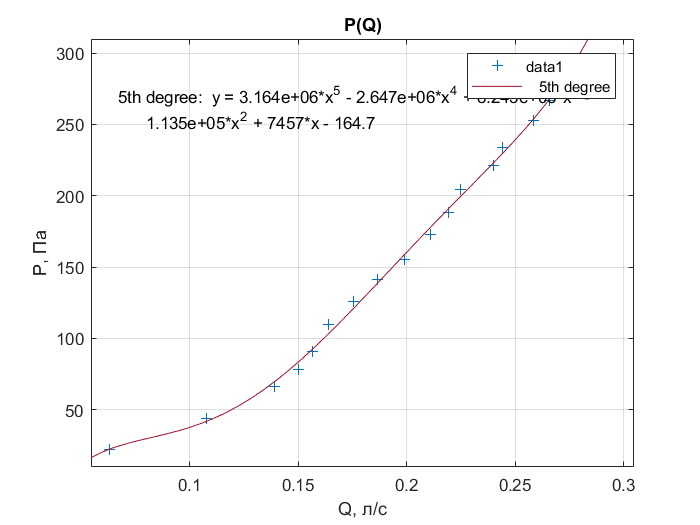
\includegraphics[width = 12 cm]{5mm}
    \caption{P(Q) для трубки 5 мм диаметром}
    \label{fig:vac}
\end{figure}

К сожалению, переходной момент смены ламинарного течения на турбулентное течение произошёл слишком быстро и в наличии только 3 точки, описывающие зависимость $P(Q)$. Так как уже ранее были найдены два значения для вязкости, не имеет смысла искать его для данной трубки с очень большой погрешностью. Поэтому просто проведём требуемые оценки (для первых пяти точек корреляция $0,912$, что уже выглядит печальным).

Границу перехода от ламинарного участка к турбулентному равна $P_{cr} = 70$ Па, что по порядку величины совпадает с ранее оценённым давлением.

Вычислим значение числа Рейнольдса $Re$ для переходной области между ламинарным и турбулентным течениями:

\begin{equation}
	Re = \frac{4 \rho Q_{cr}}{\pi d \eta} \simeq 1980
\end{equation}

\subsection{Исследование зависимости P(x)}

Для трёх различных трубок проверим выполнимость линейности давления от расстояния при ламинарном течении.

Снимая значения давлений на разных участках трубки при фиксирвоанной длине, имеем следующиее графики:

\begin{figure}[!h]
    \centering
    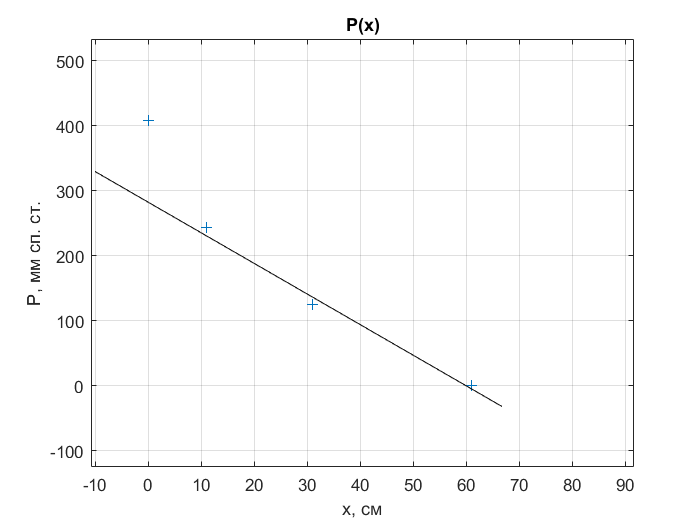
\includegraphics[width = 9 cm]{pl3}
    \caption{P(x) для трубки 3 мм диаметром}
    \label{fig:vac}
\end{figure}


\begin{figure}[!h]
    \centering
    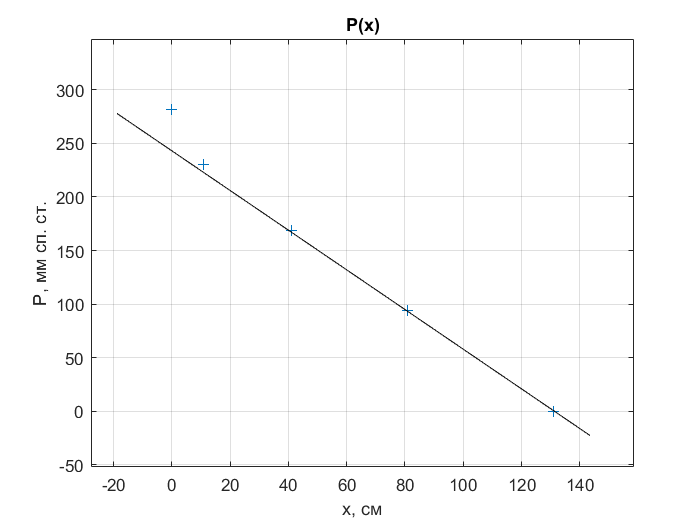
\includegraphics[width = 9 cm]{pl4}
    \caption{P(Q) для трубки 4 мм диаметром}
    \label{fig:vac}
\end{figure}

\begin{figure}[!h]
    \centering
    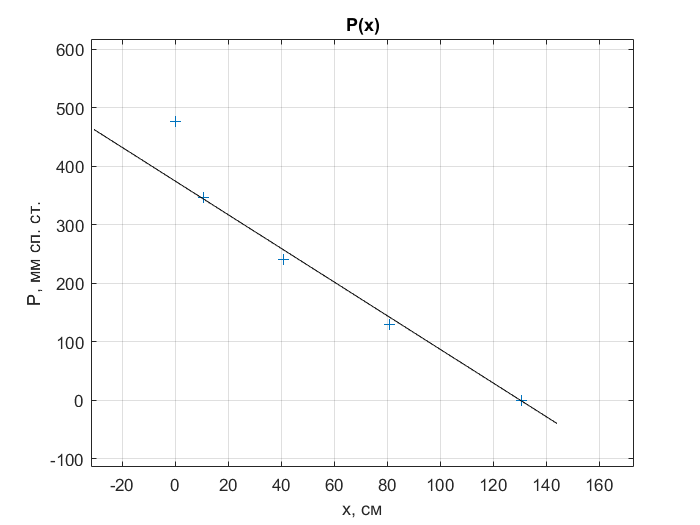
\includegraphics[width = 11 cm]{pl5}
    \caption{P(Q) для трубки 5 мм диаметром}
    \label{fig:vac}
\end{figure}
\newpage

Видно, что установление давления в начале трубы происходит быстро и графики преобретают линейный характер уже после $l_{cr} = 10$ см.

\subsection{Исследование зависимости Q(d)}

Подберём градиент давления такой, чтобы д=на всех трубках было заведомо ламинарное течение. Для трубок 4 и 5 мм выберем длину $l = 50$ см, для самой тонкой трубки $l = 30$ см.

Снимаем данные и строим график зависимости $ln(Q)(ln(d))$:

\begin{equation}
	Q(r) = C \cdot d^n \Rightarrow ln(Q) = nln(d) + C'
\end{equation}

Для ламинарного течения $\frac{\Delta P}{l}  = 1,57 \; \text{Па/м}$.

\begin{center}
\begin{tabular}{|c|c|c|c|}
\hline
$Q$, л/c & 0,0181  & 0,0581  & 0,1383  \\ \hline
$d$, мм  & 3      & 4      & 5      \\ \hline
$ln(Q)$  & -4,012 & -2,846 & -1,978 \\ \hline
$ln(d)$  & 1,0986 & 1,3731 & 1,5994 \\ \hline
\end{tabular}
\end{center}

\begin{figure}[!h]
    \centering
    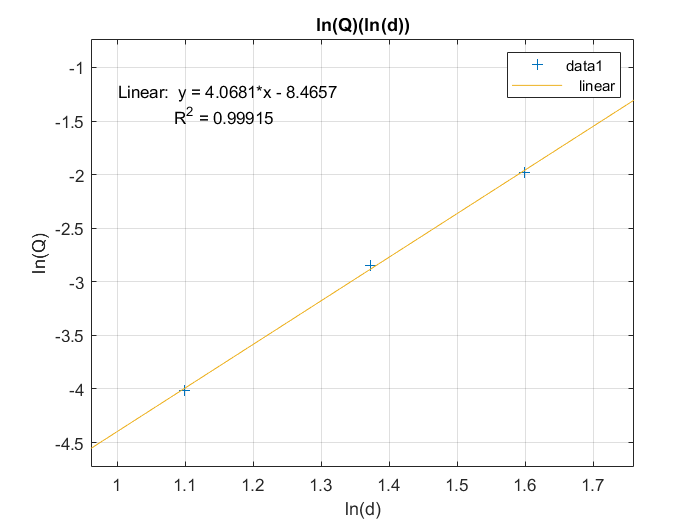
\includegraphics[width = 12 cm]{qr}
    \caption{ln(Q)(ln(d))}
    \label{fig:vac}
\end{figure}

Имеем $n = 4,0681$, $\Delta n = 0,0731$ -- формула Пуазёйля верна.

Теперь проделаем те же самые действия для турбулентного течения. Теперь возьмём $\frac{\Delta P}{l}  = 4,71 \; \text{Па/м}$.

\begin{center}
\begin{tabular}{|c|c|c|c|}
\hline
$Q$, л/c & 0,0552  & 0,1155  & 0,2031  \\ \hline
$d$, мм  & 3      & 4      & 5      \\ \hline
$ln(Q)$  & -2,897 & -2,158 & -1,594 \\ \hline
$ln(d)$  & 1,0986 & 1,3731 & 1,5994 \\ \hline
\end{tabular}
\end{center}

\begin{figure}[!h]
    \centering
    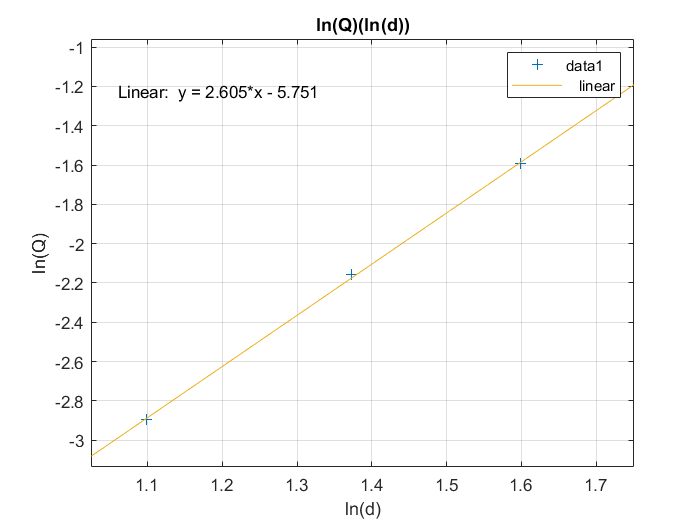
\includegraphics[width = 12 cm]{qr_turb}
    \caption{ln(Q)(ln(d))}
    \label{fig:vac}
\end{figure}

Имеем $n = 2,605$, $\Delta n = 0,0795$ -- результат практически совпадает с рассчитанным теоретически. 

\newpage 

\section{Характеристики молекул воздуха}

Ради интереса найдём длину свободного пробега из рассчитанного значения вязкости:

\begin{equation}
	\eta = \frac{1}{3}nmv \lambda = \frac{\mu}{3 N_{A}} \frac{P}{kT} \sqrt{\frac{8RT}{\pi \mu}} \lambda = \frac{P}{3}  \sqrt{\frac{8 \mu}{\pi RT}} \lambda \Rightarrow
\end{equation}

\begin{equation}
	\Rightarrow \lambda = \frac{3 \eta}{P} \sqrt{\frac{\pi RT}{8 \mu}} = 99 \; \text{нм}
\end{equation}

\begin{equation}
	\lambda = \frac{4}{\sqrt{2} n \pi d^2} = \frac{4kT}{\sqrt{2} P \pi d^2} \Rightarrow d \simeq 6,13 \cdot 10^{-10} \; \text{м}
\end{equation}



\section{Заключение}

\begin{enumerate}
	\item При выполнении данной работы были исследованы различные режимы течения газа по трубкам. На практике получена экспериментальная зависимость разницы давления в различных точках трубки в зависимости от расхода воздуха, идущего через трубку.
	\item Исследовались условия перехода течения из одного режима (ламинарного) в другой (турбулентный).
	\item Полученные зависимости разницы давлений от расхода воздуха согласуются с существующей теорией, описывающей движение газов и жидкостей в различных режимах.
	\item Определены значения вязкости воздуха для трубок различной длины. Полученные значения свопадают с табличными в пределах погрешностей.
	\item Основной вклад в погрешность итогового значения вязкости внесла погрешность измерения времени, а так же погрешности измерения давлений. Погрешности, связанные с установкой (погрешность линейных размеров установки, диаметра трубок) внесли меньший вклад в итоговое значение погрешности.
	\item Частично подтверждена теоретическая линейная зависимость падания давления с изменением расстояния от края трубки.
	\item Подтверждена формула Пуазейля для расхода газа при прохождении через трубку.
\end{enumerate}

\section{Список используемой литературы}

$\bullet$ Гладун А. Д. Лабораторный практикум по общей физике. Термодинамика и молекулярная физика\\

$\bullet$ \href{https://mipt.ru/education/chair/physics/S_II/lab/}{Описание лабораторных работ на кафедре общей физики МФТИ}

\end{document}